\documentclass{classrep}
\usepackage[utf8]{inputenc}
\frenchspacing

\usepackage{graphicx}
\usepackage[usenames,dvipsnames]{color}
\usepackage[hidelinks]{hyperref}
\usepackage{lmodern}
\usepackage{placeins}
\usepackage{url}
\usepackage{amsmath, amssymb, mathtools}
\usepackage{listings}
\usepackage{fancyhdr, lastpage}

\pagestyle{fancyplain}
\fancyhf{}
\renewcommand{\headrulewidth}{0pt}
\cfoot{\thepage\ / \pageref*{LastPage}}

%--------------------------------------------------------------------------------------%
\studycycle{Informatyka stosowana, studia dzienne, II st.}
\coursesemester{II}

\coursename{Analiza danych złożonych}
\courseyear{2021/2022}

\courseteacher{dr hab inż. Agnieszka Duraj}
\coursegroup{środa, 11:00}

\author{%
    \studentinfo[239671@edu.p.lodz.pl]{Jan Karwowski}{239671}\\
    \studentinfo[239676@edu.p.lodz.pl]{Kamil Kowalewski}{239676}\\
}

\title{Zadanie 3.: Wyjątki w strumieniach danych}

\begin{document}
    \maketitle
    \thispagestyle{fancyplain}

    \tableofcontents
    \newpage

    \section{Cel} {
        Celem zadania jest wykorzystanie wybranych algorytmów do wykrywania wzorców
        wyjątkowych dla trzech różnych strumieni danych.
    }

    \section{Zbiory danych} {
        Do przeprowadznia badań w tym zadaniu zostały wykorzystane trzy strumienie danych.
        Ich cechą wspólną jest układ kolumn, pierwszą z nich jest data pomiaru
        natomiast druga wartość. Ich struktura jest podyktowana działaniem algorytmu
        SHESD opisanego w sekcji \ref{algo_descripton}.

        Pierwszy strumień danych o nazwie \textit{AirPassengers}\cite{air_passengers}
        zawiera informacje o liczbie pasażerów samolotów w poszczególnych miesiącach w
        latach od 1949 do 1960.

        Drugi strumień danych o nazwie \textit{Alcohol sales}\cite{alcohol_sales}
        zawiera informacje o sprzedaży alkoholu w latach 1992 - 2019.

        Trzeci strumień danych o nazwie \textit{Gold price}\cite{gold_price}
        zawiera informacje o cenach złota w latach 1970 - 2020.

        Dla wszystkich trzech zbiorów, które to oryginalnie nie zawierały zauważalnych wartości
        wyjątkowych, zostały one wygenerowane sztucznie, na potrzebny eksperymentów. Dla każdego
        zbioru wybranych zostało kilka punktów, wizualnie wyraźnie odstających od głównego trendu
        strumienia danych.
    }

    \section{Implementacja} {
        Program został napisany w języku Python z wykorzystaniem bibliotek
        \textit{statsmodel}\cite{statsmodel}, \textit{sesd}\cite{sesd},
        scikit-learn\cite{sklearn} aby skorzystać z gotowych implementacji algorytmów.

        Wybranymi algorytmami są:
        \begin{itemize}
            \item ARIMA (ang. AutoRegressive Integrated Moving Average)
            \item SHESD (ang. Seasonal Hybrid Extreme Studentized Deviation)
        \end{itemize}

        Do kodu źródłowego jest dołączony skrypt \textit{run.sh} zawierający wszystkie
        kombinacja parametrów użyte do badań natomiast wyniki w postaci wykresów są
        zapisywane do plików.
    }

    \section{Opis algorytmów} \label{algo_descripton} {

        \subsection{ARIMA} {
            Algorytm \textit{ARIMA}\cite{arima} (ang. AutoRegressive Integrated Moving Average) to
            model liniowy, służący do aproksymacji danych strumieniowych (ang. time series).
            Składają się na niego właściwie dwa odrębne modele, pierwszy to model
            \textit{AutoRegressive}, który przewiduje wartość próbki jako kombinację liniową $p$
            poprzednich próbek, a drugi to model \textit{Moving Average}, który wykorzystuje
            kombinację liniową błędów przybliżenia poprzednich $q$ próbek. Oba te modele są
            połączene i dodatkowo wprowadzony jest jeszcze parametr $d$, który oznacza wielokrotność
            różnicowania strumienia danych, mającego na celu uczynienie go stacjonarnym, co jest
            niezbędne aby model ten działał poprawnie. Algorytm \textit{ARIMA} posiada
            swoją modyfikację dla danych okresowych (zawierających pewien cykl), który nazywa się
            \textit{Seasonal ARIMA (SARIMA)} i posiada on dodatkowy zestaw parametrów $P$, $Q$ i $D$
            odnoszących się do tego cyklu.

            Aby znaleźć wyjątki za pomocą tego algorytmu modeluje się najpierw strumień a następnie
            wybiera te próbki, które mają największy błąd aproksymacji.
        }

        \subsection{SHESD} {
            Algorytm \textit{SHESD}\cite{shesd_wyklad} (ang. Seasonal Hybrid Extreme
            Studentized Deviation) służy do wykrywania wyjątków w jednowymiarowych
            strumieniach danych. Parametrem wymaganych do działania algorytmu jest
            określenie górnej granicy przewidywanej wartości danego odchylenia i jest
            on zazwyczaj określany jako \textit{r}. Dla każdej próbki uznanej jako wyjątek
            wykonywany jest test \textit{ESD} tyle razy ile został zdefiniowany
            parametr \textit{r} dla każdej wartości, dla dwóch wartości odstających i
            kolejnych aż do jej faktycznego osiągnięcia. Z informacji wynika, że
            algorytm ten dobrze wyznacza wartości krytyczne oraz prawidłowo wyszukuje
            wyjątki.
        }
    }

    \section{Eksperymenty} {

        Wykonane zostały dwie serie eksperymentów, pierwsza dla algorytmu ARIMA (SARIMA) a druga,
        dla algorytmu SHESD. W przypadku algorytmu ARIMA optymalne hiperparametry zostały znalezione
        poprzez przeszukiwanie siatki, realizowane biblioteką auto-arima (\textit{pmdarima}) języka
        Python. W przypadku dwóch zbiorów o naturze cyklicznej, wykorzystany został faktycznie
        algorytm SARIMA. Dla wyszukanych hiperparametrów dobrany został eksperymentalnie próg
        (\textit{threshold}), decydujący o czułości wyszukiwania wyjątków zgodnie z warunkiem:
        \begin{equation}
            \textrm{err}^{2}_{i} > \textrm(threshold) \cdot \textrm{std}(\textrm{err}^{2})
        \end{equation}
        gdzie $\textrm{err}_{i}$ oznacza błąd aproksymacji i-tej próbki, a
        $\textrm{std}(\textrm{err}^{2})$ to odchylenie standardowe błędu średnikwadratowego
        aproksymacji całego sygnału.

        W przypadku algorytmu SHESD, to właściwie został on wykorzystany jedynie dla zbiorów o
        naturze cyklicznej, dla trzeciego zbioru (gold price) użyty został zwykły ESD. Dodatkow dla
        tego trzeciego zbioru, został on najpierw poddany operacji różnicowania.

        Na wszystkich rysunkach przedstawiających wyniki działania algorytmów, niebieska linia
        prezentuje sygnał wejściowy (strumień danych), zielone krzyżyki oznaczają punkty będące
        faktycznie wartościami odstającymi a czerwone kropki oznaczają punkty rozpoznane jako
        odstające przez dany algorytm.

        \subsection{Zbiór AirPassengers} {

            \subsubsection{ARIMA} {

                \begin{figure}[!htbp]
                    \centering
                    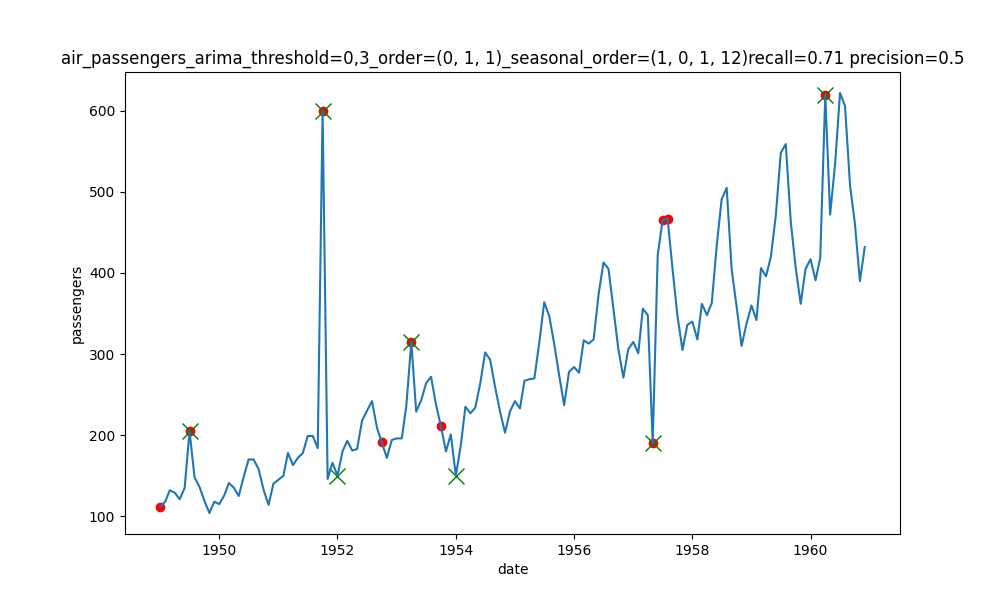
\includegraphics[width=\textwidth]{img/air_passengers_arima_threshold=0,3_order=(0,1,1)_seasonal_order=(1,0,1,12)-203749.png}
                    \caption
                    {Wykres dla zbioru AirPassengers, algorytmu ARIMA i parametrów threshold=0,3; order=(0,1,1); seasonal\_order=(1,0,1,12)}
                    \label{fig:arima_air}
                \end{figure}
                \FloatBarrier
            }

            \subsubsection{SHESD} {

                \begin{figure}[!htbp]
                    \centering
                    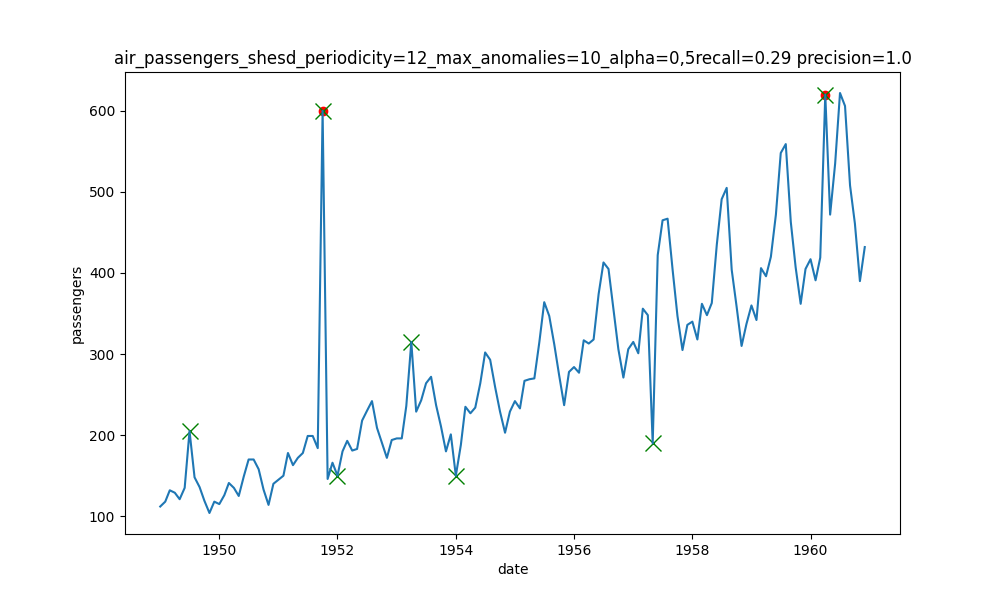
\includegraphics[width=\textwidth]{img/air_passengers_shesd_periodicity=12_max_anomalies=10_alpha=0,5-203733.png}
                    \caption
                    {Wykres dla zbioru AirPassengers, algorytmu SHESD i parametrów periodicity=12; max\_anomalies=10; alpha=0,5}
                    \label{fig:shesd_air}
                \end{figure}
                \FloatBarrier
            }
        }

        \subsection{Zbiór Alcohol sales} {

            \subsubsection{ARIMA} {

                \begin{figure}[!htbp]
                    \centering
                    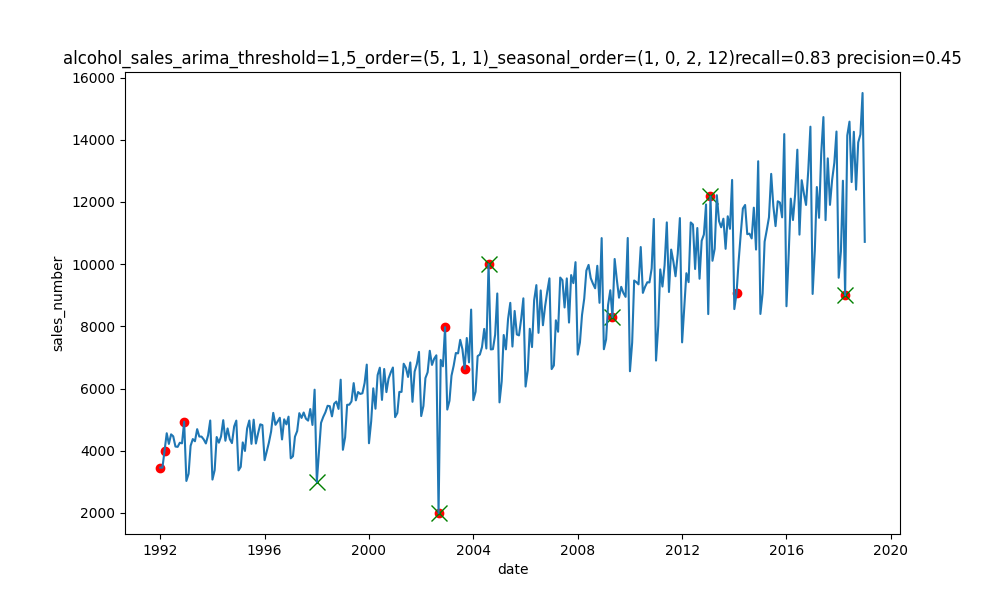
\includegraphics[width=\textwidth]{img/alcohol_sales_arima_threshold=1,5_order=(5,1,1)_seasonal_order=(1,0,2,12)-203803.png}
                    \caption
                    {Wykres dla zbioru Alcohol sales, algorytmu ARIMA i parametrów threshold=1,5; order=(5,1,1); seasonal\_order=(1,0,2,12)}
                    \label{fig:arima_alcohol}
                \end{figure}
                \FloatBarrier
            }

            \subsubsection{SHESD} {

                \begin{figure}[!htbp]
                    \centering
                    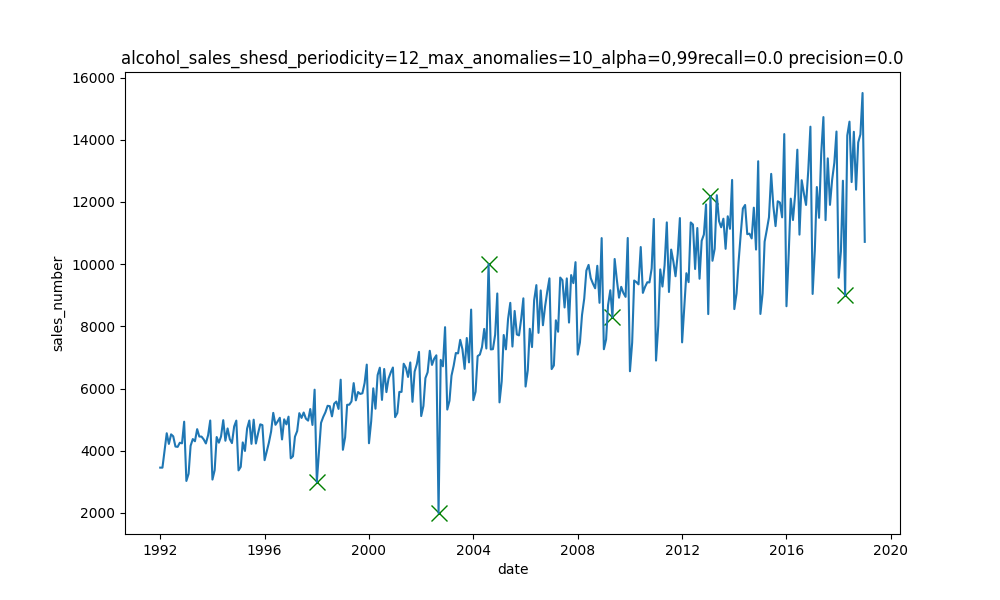
\includegraphics[width=\textwidth]{img/alcohol_sales_shesd_periodicity=12_max_anomalies=10_alpha=0,99-203739.png}
                    \caption
                    {Wykres dla zbioru Alcohol sales, algorytmu SHESD i parametrów periodicity=12; max\_anomalies=10; alpha=0,99}
                    \label{fig:shesh_alcohol}
                \end{figure}
                \FloatBarrier
            }
        }

        \subsection{Zbiór Gold price} {

            \subsubsection{ARIMA} {

                \begin{figure}[!htbp]
                    \centering
                    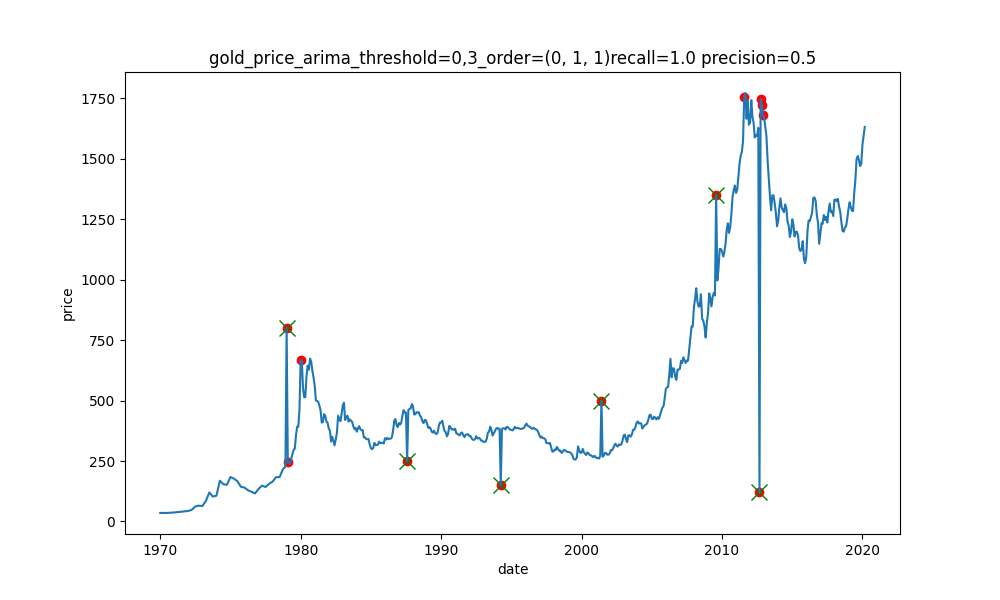
\includegraphics[width=\textwidth]{img/gold_price_arima_threshold=0,3_order=(0,1,1)-203807.png}
                    \caption
                    {Wykres dla zbioru Gold price, algorytmu ARIMA i parametrów threshold=0,3; order=(0,1,1)}
                    \label{fig:arima_gold}
                \end{figure}
                \FloatBarrier
            }

            \subsubsection{SHESD} {

                \begin{figure}[!htbp]
                    \centering
                    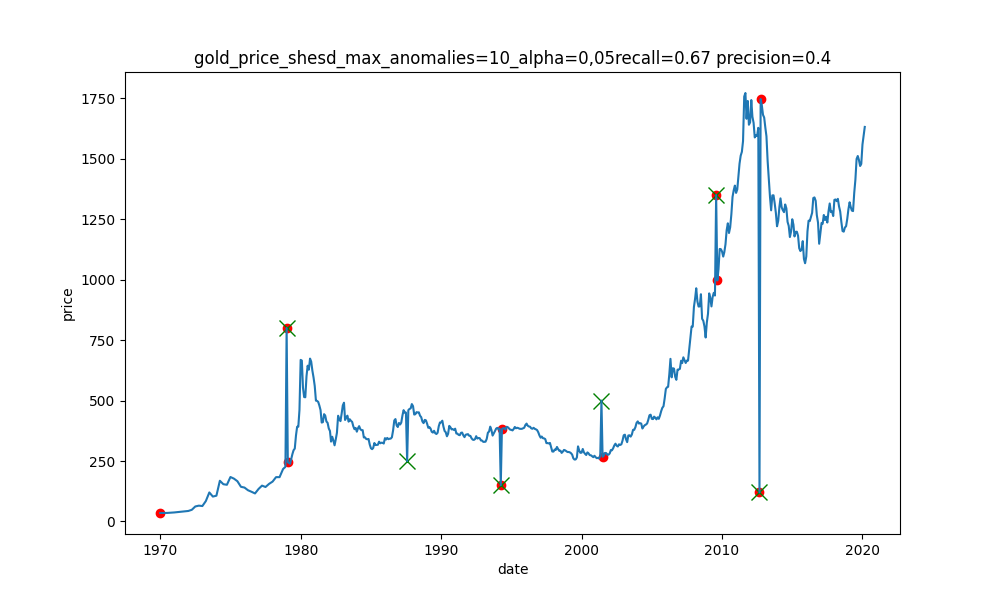
\includegraphics[width=\textwidth]{img/gold_price_shesd_max_anomalies=10_alpha=0,05-203742.png}
                    \caption
                    {Wykres dla zbioru Gold price, algorytmu SHESD i parametrów max\_anomalies=10; alpha=0,05}
                    \label{fig:shesd_gold}
                \end{figure}
                \FloatBarrier
            }
        }

        \begin{table}[!htbp]
            \centering
            \begin{tabular}{|c|c|c|c|}
                \hline
                Metoda & Zbiór danych & recall & precision \\ \hline
                shesd & air\_passengers & 0.29 & 1.0 \\ \hline
                shesd & alcohol\_sales & 0.0 & 0.0 \\ \hline
                shesd & gold\_price & 0.67 & 0.4 \\ \hline
                arima & air\_passengers & 0.71 & 0.5 \\ \hline
                arima & alcohol\_sales & 0.83 & 0.45 \\ \hline
                arima & gold\_price & 1.0 & 0.5 \\ \hline
            \end{tabular}
            \caption{Tabela z wartościami uzyskanych miar jakości}
            \label{tab:metrics}
        \end{table}
        \FloatBarrier
    }

    \section{Dyskusja i wnioski} {
        Podsumowanie wszystkich eksperymentów znajduje się w tabeli \ref{tab:metrics}. Można tutaj
        zobaczyć, że algorytm ARIMA sprawdził się lepiej niż algorytm SHESD. Dla każdego zbioru
        udało się zaznaczyć większość wyjątków (wysoki recall), chociaż w przypadku tego algorytmu
        mamy również do czynienia z wieloma fałszywie pozytywnymi oznaczeniami. Można więc
        powiedzieć, że czułość tego algorytmu jest zbyt duża. Widać to również na wszystkich
        rysunkach przedstawiających wyniki działania algorytmu ARIMA (rys. \ref{fig:arima_air},
        \ref{fig:arima_alcohol} i \ref{fig:arima_gold}). Można tutaj znaleźć dużo czerwonych kropek,
        które są wyraźnie nadmiarowe. Zachowanie to wynika z zasady działania zastosowanej metody,
        która jest oparta o dowolnie wybraną wartość progową, decydującą o czułości algorytmu.
        Jeżeli weźmie się ją zbyt mała, jak to ma miejsce w przypadku tych eksperymentów, algorytm
        wybierze prawie wszystkie wartości odstające oraz ,,przy okazji'' niektóre wartości,
        stanowiące poprawną część strumienia danych. Wynik ten można łatwo kontrolować wspomnianym
        parametrem, nie da się jednak inaczej, jak zmieniając sam model ARIMA, osiągnąć
        korzystiejszy kompromis między czułością a precyzją.

        Drugi wykorzystany model (SHESD) został stworzony z myślą o znajdowaniu wyjątków w
        strumieniu danych. Dodatkowo należy wspomnieć, że algorytm ten był tworzony w kontekście i w
        oparciu o dane rzeczywiste. Tak więc to właśnie może być główna przyczyna niepowodzenia tego
        algorytmu w przypadku wybranych/stworzonych zbiorów danych - wyjątki zostały wygenerowane
        sztucznie i z punktu widzeni tej konkretnej metody nie wyróżniają się ona dość, aby mogły
        zostać uznane za wartości odstające. Najlepsze wyniki są dla zbioru \textit{gold price},
        który jako, że nie jest cykliczny był analizowany jedynie algorytmem ESD. W zbiorze
        \textit{air passengers} udało się zlokalizować jedynie dwa wyjątki (rys.
        \ref{fig:shesd_air}) przy bardzo dużym poziomie istotności statystycznej przeprowadzanego w
        ramach tej metody testu statystycznego. Dla zbioru \textit{alcohol sales} nie udało
        się znaleźć żadnego błędu. Na rys. \ref{fig:shesh_alcohol} widać jednak, że w stosunku do
        wyników dla zbioru \textit{air passengers}, wygenerowane wyjątki zdecydowanie mniej
        wyróżniają się spośród właściwych wartości strumienia. Należy na końcu zwrócić jednak uwagę,
        że całą przewagą tej metody jest właśnie brak potrzeby szukania jej hiperparametrów i
        specjalnego dostrajania, które ma miejsce w przypadku algorytmu ARIMA.
    }

    \begin{thebibliography}{0}
        % @formatter:off
        \bibitem{statsmodel}{https://www.statsmodels.org/stable/index.html}
        \bibitem{arima}{https://www.statsmodels.org/dev/generated/statsmodels.tsa.arima.model.ARIMA.html}
        \bibitem{shesd_wyklad}{Dr hab. inż. Agnieszka Duraj. Wykrywanie wyjątków w strumieniach danych przy użyciu metod statystycznych i odległościowych}
        \bibitem{sesd}{https://pypi.org/project/sesd/}
        \bibitem{sklearn}{https://scikit-learn.org/stable/}
        \bibitem{air_passengers}{https://www.kaggle.com/rakannimer/air-passengers}
        \bibitem{alcohol_sales}{https://www.kaggle.com/bulentsiyah/for-simple-exercises-time-series-forecasting\\
        ?select=Alcohol\_Sales.csv}
        \bibitem{gold_price}{https://www.kaggle.com/arashnic/learn-time-series-forecasting-from-gold-price\\
        ?select=gold\_price\_data.csv}
        % @formatter:on
    \end{thebibliography}

\end{document}
